\begin{figure}[htbp]
	\centering
	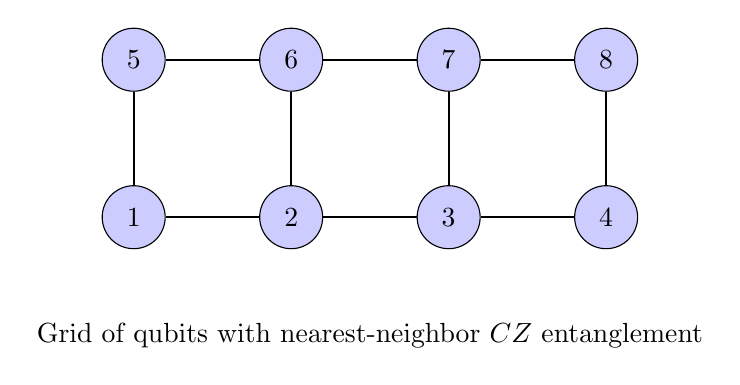
\begin{tikzpicture}
		\node[draw, circle, fill=blue!20, minimum size=0.8cm] (11) at (0,0) {1};
		\node[draw, circle, fill=blue!20, minimum size=0.8cm] (12) at (2,0) {2};
		\node[draw, circle, fill=blue!20, minimum size=0.8cm] (13) at (4,0) {3};
		\node[draw, circle, fill=blue!20, minimum size=0.8cm] (14) at (6,0) {4};
		\node[draw, circle, fill=blue!20, minimum size=0.8cm] (21) at (0,2) {5};
		\node[draw, circle, fill=blue!20, minimum size=0.8cm] (22) at (2,2) {6};
		\node[draw, circle, fill=blue!20, minimum size=0.8cm] (23) at (4,2) {7};
		\node[draw, circle, fill=blue!20, minimum size=0.8cm] (24) at (6,2) {8};

		\draw[thick] (11) -- (12) -- (13) -- (14);
		\draw[thick] (21) -- (22) -- (23) -- (24);
		\draw[thick] (11) -- (21);
		\draw[thick] (12) -- (22);
		\draw[thick] (13) -- (23);
		\draw[thick] (14) -- (24);

		\node at (3,-1.5) {Grid of qubits with nearest-neighbor $CZ$ entanglement};
	\end{tikzpicture}
	\caption{The cluster state, a 2D square lattice graph state. This is a universal resource for measurement-based quantum computation, where computation proceeds through single-qubit measurements on the entangled cluster. Cluster State: 2D square lattice graph, universal resource for one-way quantum computation.}
	\label{fig:cluster-state}
\end{figure}
